\documentclass{standalone}
\usepackage{mathpazo}
\usepackage{siunitx}
\usepackage[american voltages, american currents, american inductors]{circuitikz}
\usetikzlibrary{calc}
\newcommand*{\equal}{=}

\begin{document}
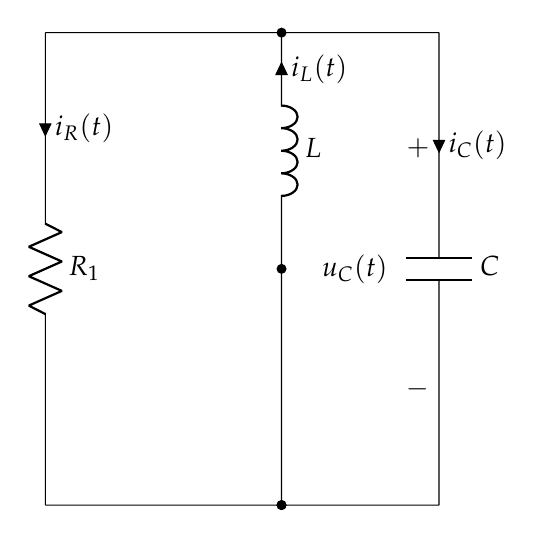
\begin{tikzpicture}
  \coordinate (A) at (0,6);
  \coordinate (B) at (3,6);
  \coordinate (C) at (5,6);
  \coordinate (D) at (0,0);
  \coordinate (E) at (3,0);
  \coordinate (F) at (5,0);
  \draw
  (A) to [short, -*] (B) to [short] (C)
  (D) to [short, -*] (E) to [short] (F)
  (A) to [R, l = $R_1$, i>^= $i_R(t)$] (D)
  (B) to [L, l = $L$, i<= $i_L(t)$] ++(0, -3)
  to [short, *-*] (E)
  (C) to [C, l= $C$, v= $u_C(t)$, i>^= $i_C(t)$] (F);
\end{tikzpicture}
\end{document}